\documentclass[a4paper]{report}
% Some basic packages
\usepackage[utf8]{inputenc}
\usepackage[T1]{fontenc}
\usepackage{textcomp}
\usepackage[english]{babel}
\usepackage{url}
\usepackage{graphicx}
\usepackage{float}
\usepackage{booktabs}
\usepackage{enumitem}

\pdfminorversion=7

% Don't indent paragraphs, leave some space between them
\usepackage{parskip}

% Hide page number when page is empty
\usepackage{emptypage}
\usepackage{subcaption}
\usepackage{multicol}
\usepackage{xcolor}

% Other font I sometimes use.
% \usepackage{cmbright}

% Math stuff
\usepackage{amsmath, amsfonts, mathtools, amsthm, amssymb}
% Fancy script capitals
\usepackage{mathrsfs}
\usepackage{cancel}
% Bold math
\usepackage{bm}
% Some shortcuts
\newcommand\N{\ensuremath{\mathbb{N}}}
\newcommand\R{\ensuremath{\mathbb{R}}}
\newcommand\Z{\ensuremath{\mathbb{Z}}}
\renewcommand\O{\ensuremath{\emptyset}}
\newcommand\Q{\ensuremath{\mathbb{Q}}}
\newcommand\C{\ensuremath{\mathbb{C}}}
\renewcommand\L{\ensuremath{\mathcal{L}}}

% Package for Petri Net drawing
\usepackage[version=0.96]{pgf}
\usepackage{tikz}
\usetikzlibrary{arrows,shapes,automata,petri}
\usepackage{tikzit}
\input{petri_nets_style.tikzstyles}

% Easily typeset systems of equations (French package)
\usepackage{systeme}

% Put x \to \infty below \lim
\let\svlim\lim\def\lim{\svlim\limits}

%Make implies and impliedby shorter
\let\implies\Rightarrow
\let\impliedby\Leftarrow
\let\iff\Leftrightarrow
\let\epsilon\varepsilon

% Add \contra symbol to denote contradiction
\usepackage{stmaryrd} % for \lightning
\newcommand\contra{\scalebox{1.5}{$\lightning$}}

% \let\phi\varphi

% Command for short corrections
% Usage: 1+1=\correct{3}{2}

\definecolor{correct}{HTML}{009900}
\newcommand\correct[2]{\ensuremath{\:}{\color{red}{#1}}\ensuremath{\to }{\color{correct}{#2}}\ensuremath{\:}}
\newcommand\green[1]{{\color{correct}{#1}}}

% horizontal rule
\newcommand\hr{
    \noindent\rule[0.5ex]{\linewidth}{0.5pt}
}

% hide parts
\newcommand\hide[1]{}

% si unitx
\usepackage{siunitx}
\sisetup{locale = FR}

% Environments
\makeatother
% For box around Definition, Theorem, \ldots
\usepackage{mdframed}
\mdfsetup{skipabove=1em,skipbelow=0em}
\theoremstyle{definition}
\newmdtheoremenv[nobreak=true]{definitie}{Definitie}
\newmdtheoremenv[nobreak=true]{eigenschap}{Eigenschap}
\newmdtheoremenv[nobreak=true]{gevolg}{Gevolg}
\newmdtheoremenv[nobreak=true]{lemma}{Lemma}
\newmdtheoremenv[nobreak=true]{propositie}{Propositie}
\newmdtheoremenv[nobreak=true]{stelling}{Stelling}
\newmdtheoremenv[nobreak=true]{wet}{Wet}
\newmdtheoremenv[nobreak=true]{postulaat}{Postulaat}
\newmdtheoremenv{conclusie}{Conclusie}
\newmdtheoremenv{toemaatje}{Toemaatje}
\newmdtheoremenv{vermoeden}{Vermoeden}
\newtheorem*{herhaling}{Herhaling}
\newtheorem*{intermezzo}{Intermezzo}
\newtheorem*{notatie}{Notatie}
\newtheorem*{observatie}{Observatie}
\newtheorem*{exe}{Exercise}
\newtheorem*{opmerking}{Opmerking}
\newtheorem*{praktisch}{Praktisch}
\newtheorem*{probleem}{Probleem}
\newtheorem*{terminologie}{Terminologie}
\newtheorem*{toepassing}{Toepassing}
\newtheorem*{uovt}{UOVT}
\newtheorem*{vb}{Voorbeeld}
\newtheorem*{vraag}{Vraag}

\newmdtheoremenv[nobreak=true]{definition}{Definition}
\newtheorem*{eg}{Example}
\newtheorem*{notation}{Notation}
\newtheorem*{previouslyseen}{As previously seen}
\newtheorem*{remark}{Remark}
\newtheorem*{note}{Note}
\newtheorem*{problem}{Problem}
\newtheorem*{observe}{Observe}
\newtheorem*{property}{Property}
\newtheorem*{intuition}{Intuition}
\newmdtheoremenv[nobreak=true]{prop}{Proposition}
\newmdtheoremenv[nobreak=true]{theorem}{Theorem}
\newmdtheoremenv[nobreak=true]{corollary}{Corollary}

% End example and intermezzo environments with a small diamond (just like proof
% environments end with a small square)
\usepackage{etoolbox}
\AtEndEnvironment{vb}{\null\hfill$\diamond$}%
\AtEndEnvironment{intermezzo}{\null\hfill$\diamond$}%
% \AtEndEnvironment{opmerking}{\null\hfill$\diamond$}%

% Fix some spacing
% http://tex.stackexchange.com/questions/22119/how-can-i-change-the-spacing-before-theorems-with-amsthm
\makeatletter
\def\thm@space@setup{%
  \thm@preskip=\parskip \thm@postskip=0pt
}


% Exercise 
% Usage:
% \exercise{5}
% \subexercise{1}
% \subexercise{2}
% \subexercise{3}
% gives
% Exercise 5
%   Exercise 5.1
%   Exercise 5.2
%   Exercise 5.3
\newcommand{\exercise}[1]{%
    \def\@exercise{#1}%
    \subsection*{Exercise #1}
}

\newcommand{\subexercise}[1]{%
    \subsubsection*{Exercise \@exercise.#1}
}


% \lecture starts a new lecture (les in dutch)
%
% Usage:
% \lecture{1}{di 12 feb 2019 16:00}{Inleiding}
%
% This adds a section heading with the number / title of the lecture and a
% margin paragraph with the date.

% I use \dateparts here to hide the year (2019). This way, I can easily parse
% the date of each lecture unambiguously while still having a human-friendly
% short format printed to the pdf.

\usepackage{xifthen}
\def\testdateparts#1{\dateparts#1\relax}
\def\dateparts#1 #2 #3 #4 #5\relax{
    \marginpar{\small\textsf{\mbox{#1 #2 #3 #5}}}
}

\def\@lecture{}%
\newcommand{\lecture}[3]{
    \ifthenelse{\isempty{#3}}{%
        \def\@lecture{Lecture #1}%
    }{%
        \def\@lecture{Lecture #1: #3}%
    }%
    \subsection*{\@lecture}
    \marginpar{\small\textsf{\mbox{#2}}}
}



% These are the fancy headers
\usepackage{fancyhdr}
\pagestyle{fancy}

% LE: left even
% RO: right odd
% CE, CO: center even, center odd
% My name for when I print my lecture notes to use for an open book exam.
% \fancyhead[LE,RO]{Gilles Castel}

\fancyhead[RO,LE]{\@lecture} % Right odd,  Left even
\fancyhead[RE,LO]{}          % Right even, Left odd

\fancyfoot[RO,LE]{\thepage}  % Right odd,  Left even
\fancyfoot[RE,LO]{}          % Right even, Left odd
\fancyfoot[C]{\leftmark}     % Center

\makeatother




% Todonotes and inline notes in fancy boxes
\usepackage{todonotes}
\usepackage{tcolorbox}

% Make boxes breakable
\tcbuselibrary{breakable}

% Verbetering is correction in Dutch
% Usage: 
% \begin{verbetering}
%     Lorem ipsum dolor sit amet, consetetur sadipscing elitr, sed diam nonumy eirmod
%     tempor invidunt ut labore et dolore magna aliquyam erat, sed diam voluptua. At
%     vero eos et accusam et justo duo dolores et ea rebum. Stet clita kasd gubergren,
%     no sea takimata sanctus est Lorem ipsum dolor sit amet.
% \end{verbetering}
\newenvironment{verbetering}{\begin{tcolorbox}[
    arc=0mm,
    colback=white,
    colframe=green!60!black,
    title=Opmerking,
    fonttitle=\sffamily,
    breakable
]}{\end{tcolorbox}}

% Noot is note in Dutch. Same as 'verbetering' but color of box is different
\newenvironment{noot}[1]{\begin{tcolorbox}[
    arc=0mm,
    colback=white,
    colframe=white!60!black,
    title=#1,
    fonttitle=\sffamily,
    breakable
]}{\end{tcolorbox}}




% Figure support as explained in my blog post.
\usepackage{import}
\usepackage{xifthen}
\usepackage{pdfpages}
\usepackage{transparent}
\newcommand{\incfig}[1]{%
    \def\svgwidth{\columnwidth}
    \import{./figures/}{#1.pdf_tex}
}

% Fix some stuff
% %http://tex.stackexchange.com/questions/76273/multiple-pdfs-with-page-group-included-in-a-single-page-warning
\pdfsuppresswarningpagegroup=1


% My name
\author{Bruno M. Pacheco}

 
\begin{document}
 
\title{Relatório 3}
\author{Bruno M. Pacheco\\
DAS 5142 - Sistemas Dinâmicos}
 
\maketitle
 
\exercise{E1}

\subsubsection*{a)}

O lugar das raízes do sistema proposto, ignorando a saturação, pode ser observado na figura \ref{fig:figures-lab3_1_rlocus-pdf}.

\begin{figure}[H]
    \centering
    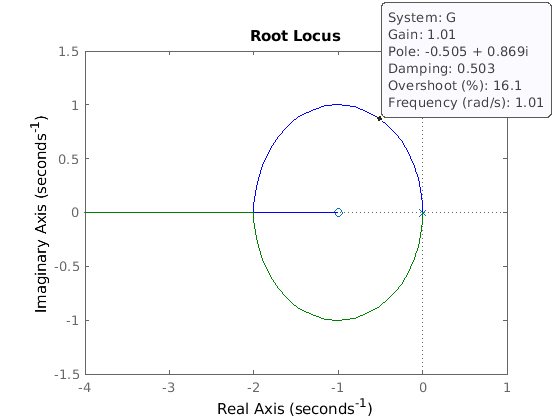
\includegraphics[width=0.6\textwidth]{figures/lab3_1_rlocus.png}
    \caption{Lugar das raízes do sistema, ignorando a saturação.}
    \label{fig:figures-lab3_1_rlocus-pdf}
\end{figure}

Nota-se que, para $k>0$, o sistema é estável. Além disso, para o ganho proposto, tem-se um par de polos complexos conjugados.

\subsubsection*{b)}

Utilizou-se a construção visível na figura \ref{fig:figures-lab3_1_simulink_model-png} no \emph{Simulink} para simular o comportamento do sistema com saturação.

\begin{figure}[H]
    \centering
    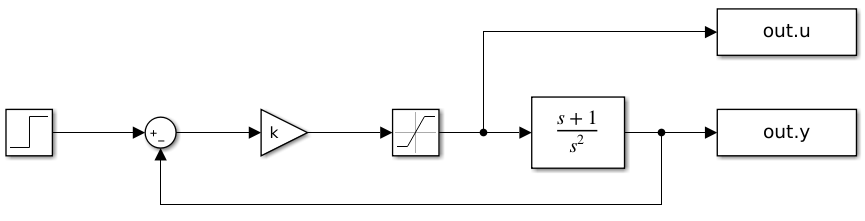
\includegraphics[width=0.6\textwidth]{figures/lab3_1_simulink_model.png}
    \caption{Modelo do sistema proposto no software \emph{Simulink}.}
    \label{fig:figures-lab3_1_simulink_model-png}
\end{figure}

A simulação foi executada aplicando um degrau na referência no instante inicial e observando os sinais de controle (após saturação) e de saída. Os resultados das simulações para os diferentes valores de referência podem ser observados na figura \ref{fig:figures-lab3_1_saturation-png}.

\begin{figure}[H]
    \centering
    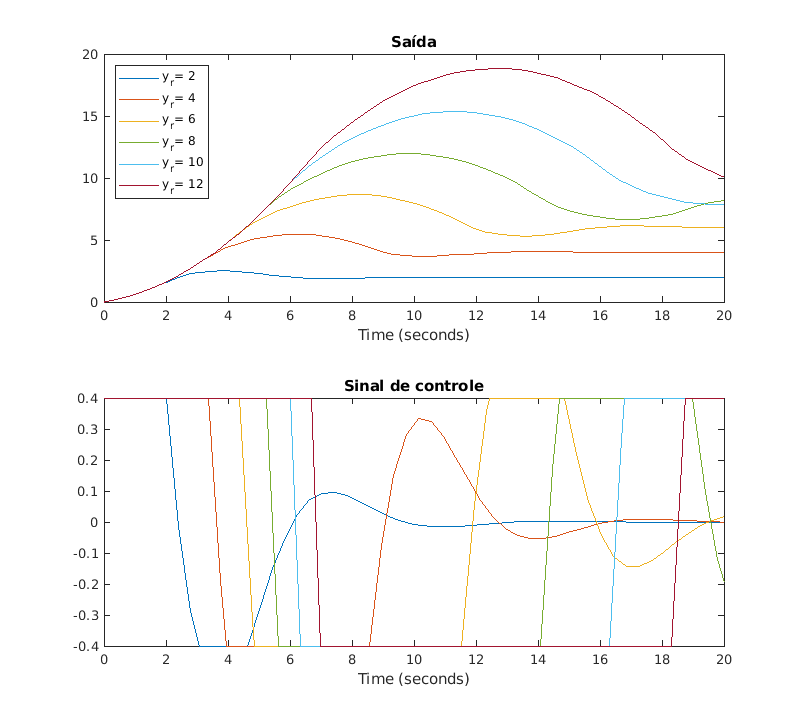
\includegraphics[width=0.8\textwidth]{figures/lab3_1_saturation.png}
    \caption{Resposta do sistema a diferentes sinais tipo degrau na referência.}
    \label{fig:figures-lab3_1_saturation-png}
\end{figure}

\subsubsection*{c)}

Pelo modelo de variáveis de estado fornecido, sabemos que os dois estados são 
\begin{align*}
    x_1(t) = \int x_2(t) \\
    x_2(t) = \int u(t)
\end{align*}
, ou seja, podemos construir o sistema da forma visível na figura \ref{fig:figures-lab3_1_state_space_model-png}, utilizando os pontos destacados para observar a trajetória dos estados do sistema.

\begin{figure}[H]
    \centering
    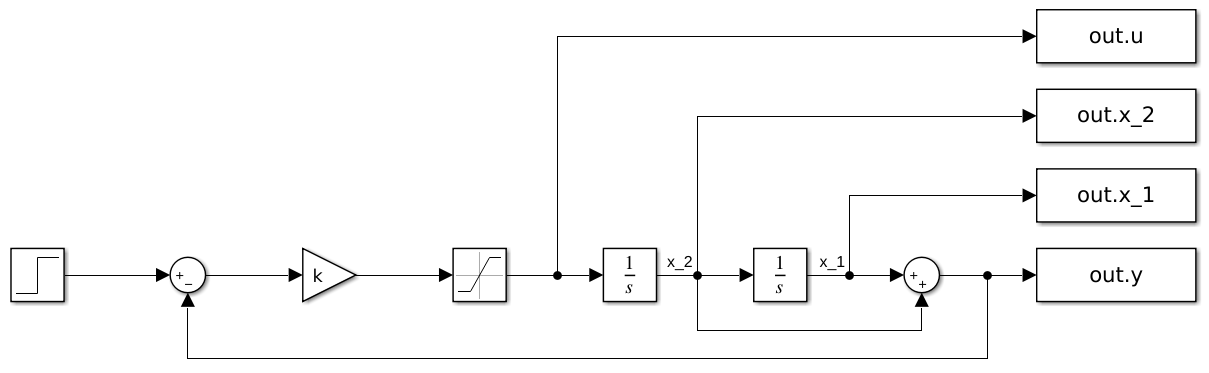
\includegraphics[width=0.6\textwidth]{figures/lab3_1_state_space_model.png}
    \caption{Modelo do sistema por variáveis de estado.}
    \label{fig:figures-lab3_1_state_space_model-png}
\end{figure}

Assim, o comportamento do sistema pode ser observada na figura \ref{fig:figures-lab3_1_state_space_response-png}.

\begin{figure}[H]
    \centering
    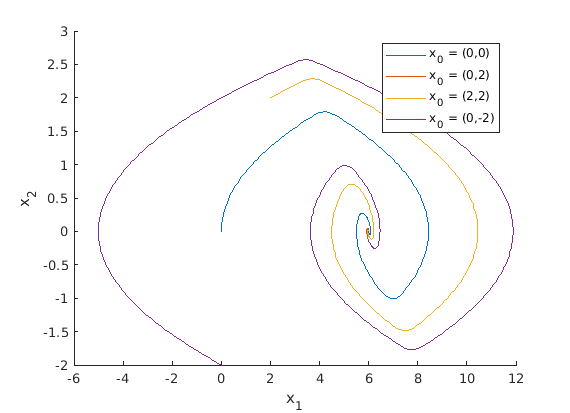
\includegraphics[width=0.8\textwidth]{figures/lab3_1_state_space_response.png}
    \caption{Trajetória dos estados para diferentes condições iniciais, utilizando uma referência degrau $y_r = 6$.}
    \label{fig:figures-lab3_1_state_space_response-png}
\end{figure}

\subsubsection*{d)}

Pode-se observar nas trajetórias dos estados o que já se esperava pelo lugar das raízes: o sistema se torna estável com o ganho estabelecido. Quanto a convergência, observa-se que, conforme a referência se distancia da origem, o sinal de controle se torna mais oscilatório, atingindo mais e mais a região de saturação, enquanto a saída caracteriza-se por um \emph{settling time} maior e mais oscilação. A resposta foi conforme o esperado, uma vez que a saturação impede o sistema de receber o sinal de controle necessário para se deslocar rapidamente para o ponto de referência, ao mesmo tempo que também impede uma resposta que possa estabilizar o sistema uma vez que uma grande "velocidade" de deslocamento dos estados é atingida. Uma forma de modelar essa intuição da saturação é através de um ganho fracionário inversamente proporcional à amplitude do sinal de referência, ou seja, quanto maior o sinal de referência é em relação à condição inicial, maior o impacto da saturação na redução do ganho.

\exercise{E2}

\subsubsection*{a)}

Pela trajetória das raízes visível na figura \ref{fig:figures-lab3_2_rlocus-pdf}, vê-se que para ganho aproximadamente menores que $0,5$, o sistema apresenta polos com parte real positiva, ou seja, é instável.

\begin{figure}[H]
    \centering
    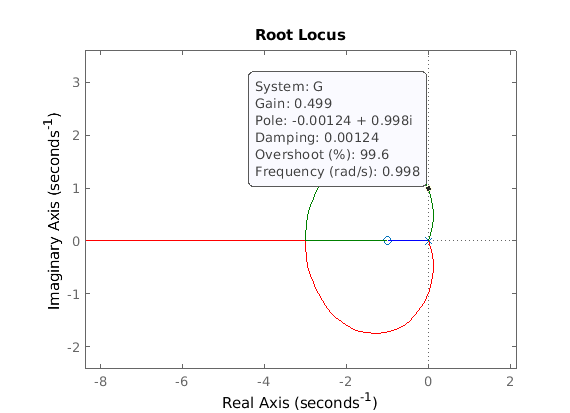
\includegraphics[width=0.6\textwidth]{figures/lab3_2_rlocus.png}
    \caption{Lugar das raízes do sistema.}
    \label{fig:figures-lab3_2_rlocus-pdf}
\end{figure}

\subsubsection*{b)}

A resposta do sistema e o comportamento do sinal de controle pode ser observado na figura \ref{fig:figures-lab3_2_saturation-png}.

\begin{figure}[H]
    \centering
    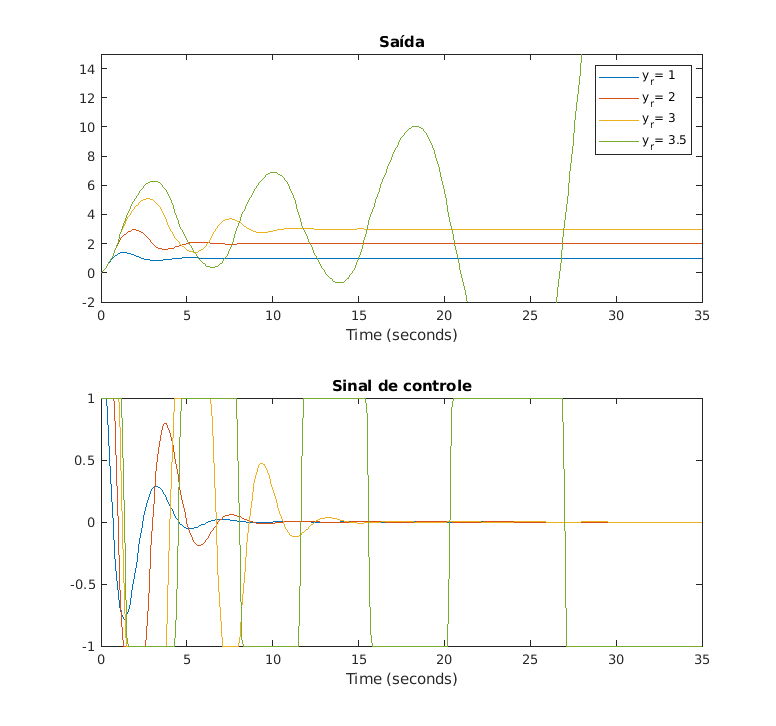
\includegraphics[width=0.8\textwidth]{figures/lab3_2_saturation.png}
    \caption{Resposta do sistema a diferentes sinais tipo degrau na referência.}
    \label{fig:figures-lab3_2_saturation-png}
\end{figure}

\subsubsection*{c)}

Para modelar o sistema proposto por variáveis de estado, selecionou-se as seguintes variáveis:
\begin{align*}
    x_1 = \int x_2 \\
    x_2 = \int x_3 \\
    x_3 = \int u \\
    y = x_1 + 2x_2 + x_3 \\
.\end{align*}
Nota-se que, em regime permanente, $y(t)\to x_1(t)$. Assim, a realização desse sistema pode ser observada na figura \ref{fig:figures-lab3_2_simulink_model-png}.

\begin{figure}[H]
    \centering
    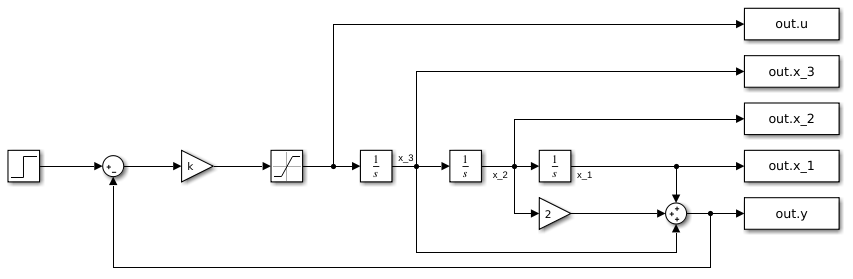
\includegraphics[width=0.6\textwidth]{figures/lab3_2_simulink_model.png}
    \caption{Modelo do sistema por variáveis de estado no software \emph{Simulink}.}
    \label{fig:figures-lab3_2_simulink_model-png}
\end{figure}

Com o modelo realizado, o sistema foi simulado com condições iniciais nulas e os valores de referência propostos. As trajetórias podem ser observadas na figura \ref{fig:figures-lab3_2_state_space_response-png}.

\begin{figure}[H]
    \centering
    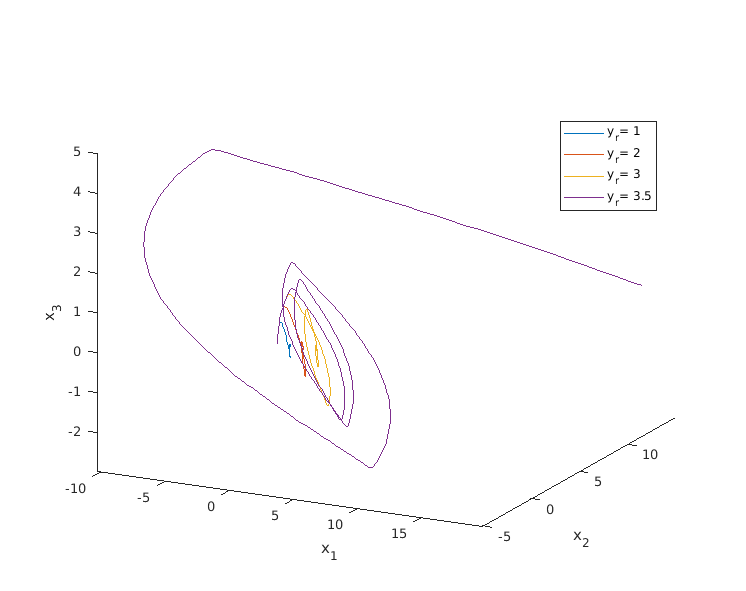
\includegraphics[width=0.8\textwidth]{figures/lab3_2_state_space_response.png}
    \caption{Trajetória dos estados para diferentes referências, com condição inicial nula.}
    \label{fig:figures-lab3_2_state_space_response-png}
\end{figure}

\subsubsection*{d)}

Sabe-se que a saturação pode ser aproximada por um ganho fracionário em função da amplitude da diferença entre a condição inicial e a referência, ou seja, para grandes amplitudes na referência, tem-se um ganho do controlador cada vez menor. Pode-se demonstrar isso através da resposta do sistema para uma condição inicial diferente, mais próxima da referência, na figura \ref{fig:figures-lab3_2_ci_3-png}.

\begin{figure}[H]
    \centering
    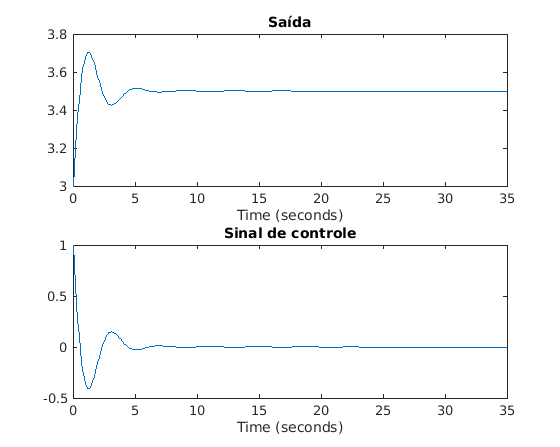
\includegraphics[width=0.8\textwidth]{figures/lab3_2_ci_3.png}
    \caption{Simulação do sistema com $y_r=3.5$ e $x_{1_0}=3$.}
    \label{fig:figures-lab3_2_ci_3-png}
\end{figure}

Pelo observado através do lugar das raízes, tem-se, na prática, uma aproximação dos polos do sistema da zona instável através da redução do ganho causada pelo aumento da amplitude da referência em conjunto com a saturação.

\exercise{E3}

\subsubsection*{a)}

Observando a trajetória dos polos do sistema, visível na figura \ref{fig:figures-lab3_3_rlocus-png}, é possível afirmar que um ganho aproximadamente superior à 0,2 leva o sistema à instabilidade, com dois polos complexos conjugados no semiplano direito.

\begin{figure}[H]
    \centering
    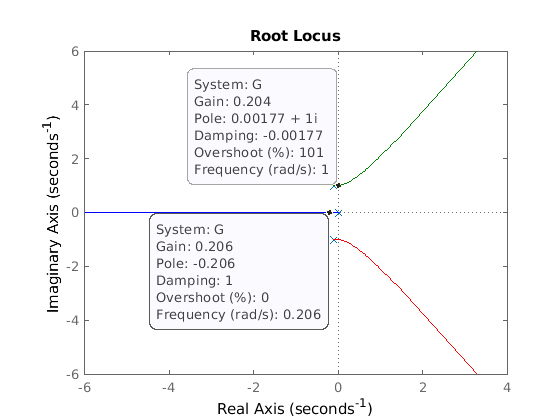
\includegraphics[width=0.8\textwidth]{figures/lab3_3_rlocus.png}
    \caption{Lugar das raízes do sistema.}
    \label{fig:figures-lab3_3_rlocus-png}
\end{figure}

\subsubsection*{b)}

Através do software \emph{Simulink}, simulou-se a resposta do sistema para diferentes referências. O resultado pode ser observado na figura \ref{fig:figures-lab3_3_saturation-png}.

\begin{figure}[H]
    \centering
    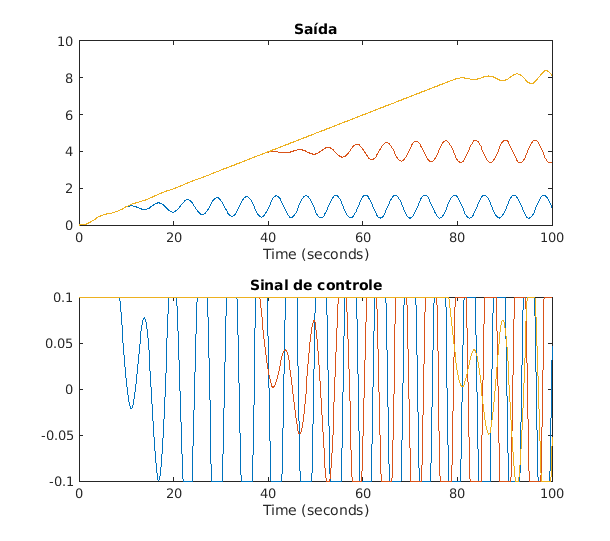
\includegraphics[width=0.8\textwidth]{figures/lab3_3_saturation.png}
    \caption{Resposta do sistema a diferentes sinais tipo degrau na referência.}
    \label{fig:figures-lab3_3_saturation-png}
\end{figure}

\subsubsection*{c)}

Para converter o sistema para um modelo em variáveis de estado, primeiro determinou-se a expressão da saída no domínio do tempo, \[
    \dddot{y}(t) + 0,2\ddot{y}(t) + \dot{y}(t) = u(t)
\] e escolheu-se os estados como \[
\begin{cases}
    \bm{x}(t) = \begin{bmatrix} y(t) \\ \dot{y}(t) \\ \ddot{y}(t) \end{bmatrix} 
\end{cases}
\], construindo o sistema, então, na forma canônica controlável da seguinte forma: \[
\begin{cases}
    \dot{x}_1(t) = x_2(t) \\
    \dot{x}_2(t) = x_3(t) \\
    \dot{x}_3(t) = -0,2x_3(t) - x_2(t) +u(t)
\end{cases}
\].

Esse sistema foi realizado conforme visível na figura \ref{fig:figures-lab3_3_state_space_model-png}.

\begin{figure}[H]
    \centering
    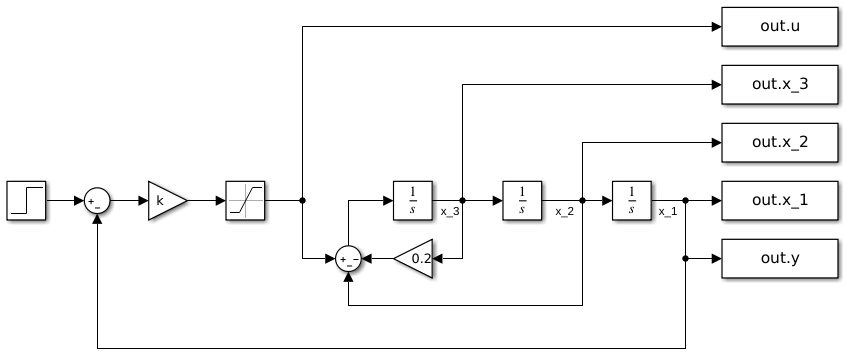
\includegraphics[width=0.6\textwidth]{figures/lab3_3_state_space_model.png}
    \caption{Modelo do sistema por variáveis de estado.}
    \label{fig:figures-lab3_3_state_space_model-png}
\end{figure}

A resposta do sistema simulado pode ser observada na figura \ref{fig:figures-lab3_3_state_space_response-png}. Notamos que a resposta oscilatória do sistema é presente não só na saída ($x_1$), como também nas outras variáveis de estado. Também é possível observar a existência de um ciclo limite estável em torno do ponto de equilíbrio desejado.

\begin{figure}[H]
    \centering
    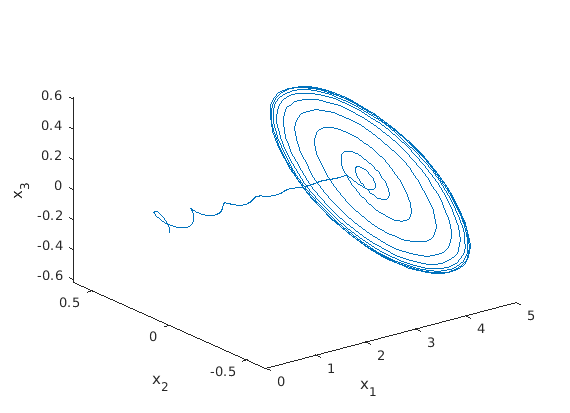
\includegraphics[width=0.8\textwidth]{figures/lab3_3_state_space_response.png}
    \caption{Trajetória dos estados para $y_r=4$, com condição inicial nula.}
    \label{fig:figures-lab3_3_state_space_response-png}
\end{figure}

\subsubsection*{d)}

Projetou-se, então, um filtro $N(s)$ de tal forma que possua dois zeros próximos aos polos conjugados originais do sistema, atraindo os polos para o SPE, e dois polos rápidos para não alterar a dinâmica do sistema. Projetou-se o filtro da seguinte forma: \[
    N(s) = \frac{200(s^{2}+0.2s+0.5}{(s+10)^2}
\].

Confirmou-se a eficácia do filtro através da simulação. A resposta do sistema pode ser observada na figura \ref{}.

\begin{figure}[H]
    \centering
    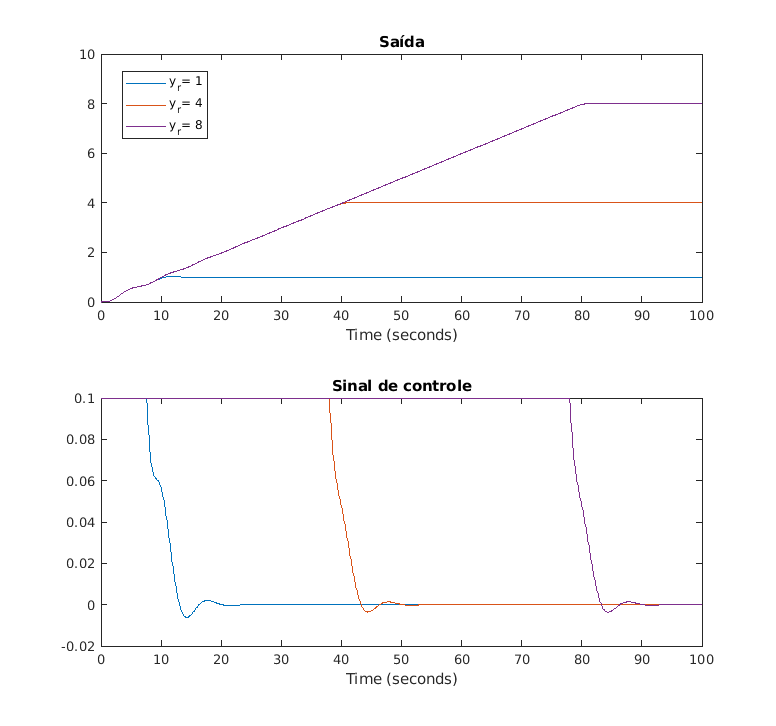
\includegraphics[width=0.8\textwidth]{figures/lab3_3_filter.png}
    \caption{Resposta do sistema com filtro.}
    \label{fig:figures-lab3_3_filter-png}
\end{figure}

\end{document}
